% % foi necessário encontrar um modelo do robot a ser utilizado - UR10e que se encontra no IRIS lab
% To successfully develop the XR application for controlling the UR10e robot, it was essential to identify a model that closely mirrors 
% the actual robot. The Unity Robotics Hub \footnote{Unity Technologies \url{https://github.com/Unity-Technologies/Unity-Robotics-Hub} 
% Accessed: 2024-02-02} facilitates the integration of robotics into Unity projects via the URDF-Importer package 
% \footnote{Unity Technologies \url{https://github.com/Unity-Technologies/URDF-Importer} Accessed: 2024-02-02}. 
% However, challenges arose when attempting to import the UR10e \textit{.urdf} model into the Unity environment. To overcome this, 
% a UR10 model, sourced from a GitHub repository \footnote{PositronicsLab \url{https://github.com/PositronicsLab/reveal_packages/tree/master/industrial_arm/scenario/models/urdf/ur10} Accessed: 2024-02-05} 
% was used, due to its resemblance to the UR10e robot. This was discussed with the educators overseeing the dissertation development, 
% and it was agreed that this approach would not pose any issues.

% In the figure \ref{f:ur10_marker_unity} it is possible to see the digital UR10 model positioned related to the aruco marker 
% (\ref{f:aruco_marker}), in a simulated Unity environment.
% \begin{figure}[h]
% \centering
% 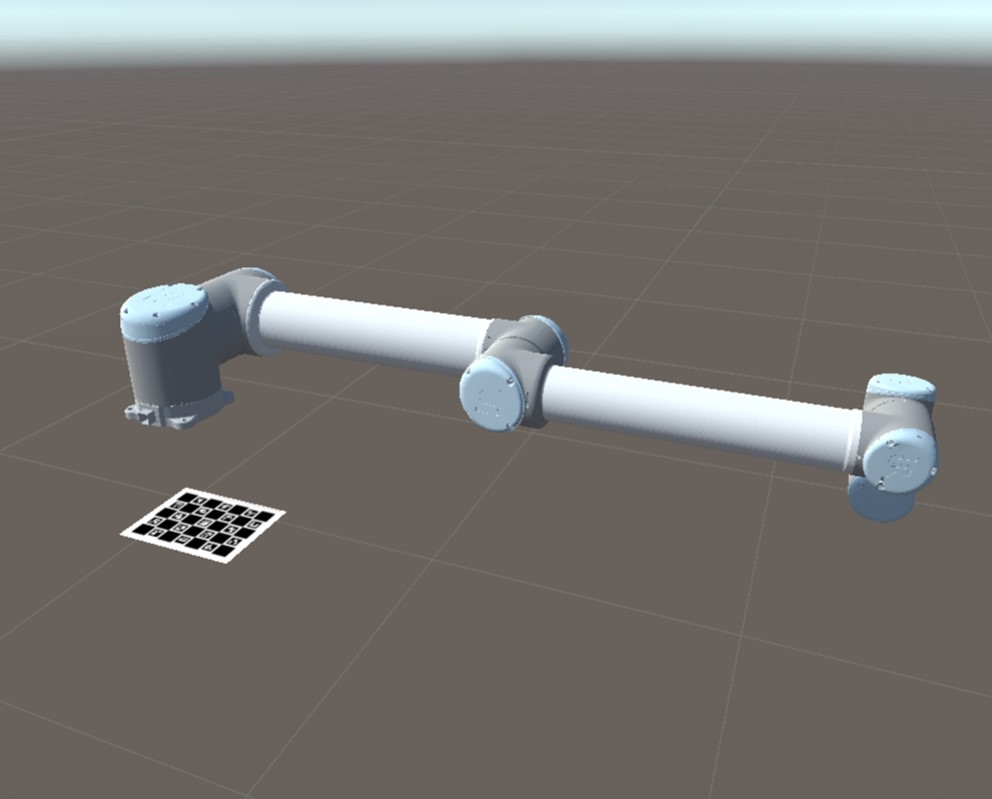
\includegraphics[width=0.6\textwidth]{figs/robot_marker_unity.jpg}
% \caption{Digital UR10 model related to the aruco marker, on Unity environment}
% \label{f:ur10_marker_unity}
% \end{figure}
